\chapter{Actividades Desarrolladas}\label{cap:actividades}
En esta sección se incluye una descripción pormenorizada de las actividades desarrolladas durante la Práctica Supervisada.

\section{Objetivos}
\subsection{Objetivo General}
Implementar un Pipeline de DevOps para aplicaciones Internet of Things (IoT) con el dispositivo ESP32.
\subsection{Objetivos Específicos}
\begin{enumerate}
\item Revisión de documentación de DevOps aplicada a IoT.
\item Elegir las herramientas para la construcción del pipeline.
\item Implementar cada etapa que compone el pipeline.
\item Desarrollar una aplicación IoT sencilla utilizando el pipeline implementado.
\item Documentar de forma incremental el trabajo realizado.
\end{enumerate}

\newpage
\section{Metodología}
\subsection{Investigación}
En primer lugar se comenzó investigando sobre la cultura DevOps, las prácticas continuas que se mencionan en el \nameref{cap:marco_teorico}, obteniendo la información a partir de documentación, artículos científicos a los cuales se hace referencia, y la lectura del libro \textit{The DevOps Handbook} \cite{DevOpsHandbook}, que menciona aspectos acerca de cómo surgió esta cultura y cuáles son las problemáticas que viene a solucionar. 

Se siguió además un curso libre y gratuito de prácticas DevOps en YouTube \href{https://www.youtube.com/watch?v=wdFwjWyF47g&list=PLnf4-vBnJ1n1Es3RyaqeIzprp4xUivflP}{(enlace al curso)}, de índole teórico-práctico, que resultó útil para conocer conceptos y herramientas como la \textbf{contenerización con Docker}, la creación de \textbf{Pipelines con GitHub Actions}, entre otras actividades que se detallan en el presente informe. 

\subsection{Dispositivo ESP32}
El dispositivo IoT elegido para trabajar es el \textbf{microcontrolador ESP32}. Se trata de un dispositivo pequeño, de bajo costo y de bajo consumo, cuyas principales prestaciones son la \textbf{conectividad WiFi} y \textbf{Bluetooth}. Su procesador posee 2 núcleos que trabajan a una frecuencia de hasta 240 MHz, entre otras características que se detallan en la siguiente tabla.

\begin{table}[h]
\begin{center}
\begin{tabular}{ll}
\hline
\multicolumn{1}{|l|}{\textbf{Fabricante}} & \multicolumn{1}{l|}{Espressif} \\ \hline
\multicolumn{1}{|l|}{\textbf{Fecha de Lanzamiento}} & \multicolumn{1}{l|}{05/09/2016} \\ \hline
\multicolumn{1}{|l|}{\textbf{Procesador}} & \multicolumn{1}{l|}{Tensilica Xtensa LX6} \\ \hline
\multicolumn{1}{|l|}{\textbf{Frecuencia}} & \multicolumn{1}{l|}{160 MHz (240MHz overclock)} \\ \hline
\multicolumn{1}{|l|}{\textbf{Alimentación}} & \multicolumn{1}{l|}{3.3 VDC} \\ \hline           
\end{tabular}
\caption{Características de ESP32}
\label{tab:car-esp32}
\end{center}
\end{table}

En concreto, este microcontrolador se vende en diferentes placas de desarrollo, con diferencias en los pines de \textbf{General Purpose Input Output (GPIO)}, y diferencias de tamaño. Es decir, se venden diferentes placas que incorporan el mismo microcontrolador ESP32, con diferencias en los pines que disponen.

La placa que se adquirió es la \textbf{“NodeMCU32S”}, que se consigue fácilmente para comprar online y dispone de 35 pines, ideal para trabajar en una protoboard y hacer pruebas. Además, dispone un conector microUSB, para poder conectarse a la PC e implementar el programa.

\begin{figure}[H]
    \centering
    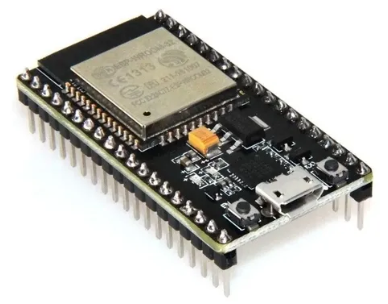
\includegraphics[width=0.6\textwidth]{fig/esp32_1.png}
    \caption{Placa NodeMCU32S.}
    \label{fig:esp32_1}
\end{figure}

Para más información sobre este dispositivo se puede consultar su datasheet en el siguiente enlace: \href{https://docs.ai-thinker.com/_media/esp32/docs/nodemcu-32s_product_specification.pdf}{Datasheet NodeMCU32s}

\subsection{Aplicación}
Se construyó una aplicación, lo más sencilla posible, para familiarizarse con la placa, con qué herramientas se puede trabajar, y qué lenguaje de programación resulta la mejor opción para este trabajo.

Se optó por crear el clásico \textbf{LED intermitente}, codificado en \textbf{lenguaje C}, que parpadea a una determinada frecuencia, observable empíricamente en el LED que trae integrado el microcontrolador. 

Cuando se desee hacer un cambio en la aplicación, lo más sencillo será modificar la frecuencia de intermitencia del LED, volver a cargar el código en la placa, y observar el cambio de frecuencia efectuado. A continuación se presenta el código \ref{cod:blinkled} de ejemplo para esta aplicación simple.

\newpage
\begin{lstlisting}[language=C, caption={BlinkLED}, label={cod:blinkled}, captionpos=b]
#include <driver/gpio.h>
// Include FreeRTOS for delay
#include <freertos/FreeRTOS.h>
#include <freertos/task.h>
#define LED 2 // LED connected to GPIO2
#define DELAY 500 // delay in ms to toggle LED state
int app_main() {
    // Configure pin
    gpio_config_t io_conf;
    io_conf.intr_type = GPIO_PIN_INTR_DISABLE;
    io_conf.mode = GPIO_MODE_OUTPUT;
    io_conf.pin_bit_mask = (1ULL << LED);
    io_conf.pull_down_en = 0;
    io_conf.pull_up_en = 0;
    gpio_config(&io_conf);
    // Main loop
    while(true) {
        gpio_set_level(LED, 0);
        vTaskDelay(pdMS_TO_TICKS(DELAY));
        gpio_set_level(LED, 1);
        vTaskDelay(pdMS_TO_TICKS(DELAY));
    }
}
\end{lstlisting}
(Código basado en el ejemplo: \href{https://techoverflow.net/2020/04/09/platformio-esp-idf-esp32-blink-example/}{PlatformIO ESP-IDF ESP32 Blink})

En el código, se observa que las primeras líneas incluyen dependencias importantes de mencionar:
\begin{itemize}
\item \textbf{gpio.h}: Permite acceder a los pines GPIO, y leer o escribir en ellos, entre otras funcionalidades.
\item \textbf{FreeRTOS.h}: Módulo principal del Sistema Operativo de tiempo real \href{https://www.freertos.org/}{FreeRTOS}, que permite gestionar los recursos del microcontrolador y crear tareas con tiempos límites.
\item \textbf{task.h}: Módulo de tareas de FreeRTOS.
\end{itemize}

A partir de la línea 8 del código, se configuran los pines GPIO para poder escribir en el LED integrado de la ESP32, y a partir de la línea 16 se tiene el bucle principal, que se repite indefinidamente, alternando el estado del LED cada \textbf{DELAY [ms]}, en este caso cada 500 [ms] pero puede modificarse fácilmente en la linea 6, es decir en su definición. La función \textbf{pdMS\_TO\_TICKS()}, convierte su parámetro de milisegundos a ticks, que es la manera de contabilizar el tiempo que utiliza \href{https://www.freertos.org/}{FreeRTOS}.

\subsection{PlatformIO}
La primera dificultad encontrada fue al cargar el programa a la placa. Para esta tarea, el fabricante brinda el software, llamado \textbf{Espressif IDF (IoT Development Framework)}, el cual usa scripts de Python para crear y gestionar proyectos. Luego de algunos intentos fallidos, se investigó una herramienta que facilita el proceso de subir el código a la placa, llamada \textbf{PlatformIO}.

\textbf{\href{https://platformio.org/}{PlatformIO}} es un framework destinado al trabajo con dispositivos IoT, soporta aproximadamente 1400 placas de desarrollo, incluyendo la \textbf{ESP32 tipo NodeMCU32S}, que se usa en este proyecto. Se puede instalar como una extensión de \textbf{Visual Studo Code}, uno de los entornos de desarrollo más populares en la actualidad, lo que resulta muy cómodo para trabajar.

Cabe destacar que PlatformIO hace uso del framework Espressif IDF, por lo tanto ayuda a crear una capa de abstracción y facilitar la creación de un proyecto, el acceso a las dependencias, la compilación y la subida del programa al dispositivo con un simple click en el botón \textbf{Build and Upload}.

Gracias a estas facilidades, se logró subir el código del ejemplo \ref{cod:blinkled} con facilidad a la placa. La figura \ref{fig:esp32_2} es una fotografía de la placa haciendo parpadear el LED integrado con éxito.

\begin{figure}[H]
    \centering
    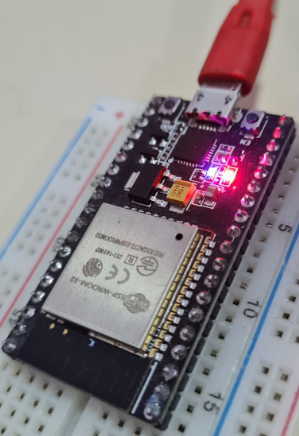
\includegraphics[width=0.5\textwidth]{fig/esp32_2.png}
    \caption{LED intermitente.}
    \label{fig:esp32_2}
\end{figure}

\subsection{Control de Versiones}
Llegado a este punto, es vital contar con una herramienta de control de versiones, para facilitar el trabajo colaborativo y poder volver atrás en caso de introducir errores importantes. Para lograr este objetivo se creó un \textbf{repositorio de Git}, que se aloja en la nube gracias a \textbf{GitHub} o \textbf{GitLab}, las dos plataformas más populares para alojar repositorios de la actualidad.

Con motivos de aprendizaje, se crearon repositorios en ambas plataformas, GitHub y GitLab, ambas son alternativas y el único propósito de subir el mismo contenido a ambas es poder diferenciar las herramientas que ofrece cada una para determinar cuál es mejor para este proyecto.

Luego de investigar y experimentar, \textbf{se decidió continuar con GitHub}, porque resulta más sencillo para aprender e incluye todas las características que necesitamos, siendo la más importante \textbf{GitHub Actions}, que permite crear workflows con secuencias de acciones a ejecutar ante determinados eventos, lo cual se detalla en secciones subsiguientes. 

El repositorio de GitHub se puede encontrar en \url{https://github.com/FeedehC/pipeline-esp32}. Al ingresar al enlace del repositorio se puede ver un README con una guía paso a paso para implementar el pipeline, permitiendo a otros desarrolladores tomar este código y usarlo en sus proyectos IoT. 

Este proyecto es considerado \textbf{Open Source}. Se incentiva la participación haciendo pruebas y realizando aportes, como así también la detección y corrección de errores mediante \textbf{GitHub issues}. 

\subsection{Continuous Integration (CI)}
El próximo paso es añadir CI al proyecto, para esto se usan \textbf{GitHub Actions}, una característica de GitHub que permite crear \textbf{Workflows}.

El término \textbf{Workflow} consiste en un flujo de trabajo, declarado en código YAML, que define distintas tareas (o \textbf{"Jobs"}), ante qué eventos se disparan los Jobs, y qué acciones se llevan a cabo en cada job. Opcionalmente los jobs pueden incluir pasos (o \textbf{"Steps"}) que indican el orden de las instrucciones dentro del job. A su vez, los jobs pueden ejecutarse en paralelo o indicar que para que inicie un job debe terminar otro, y de esta manera crear el mencionado workflow.

En cambio, el término \textbf{Pipeline}, hace alusión a un conjunto de etapas más lineal y más rápido que un workflow, sin embargo, es habitual usar estos términos de forma intercambiable. En los párrafos que siguen se usa el término Workflow porque así se llaman en GitHub Actions.

Una vez creado el workflow, se indica el evento que lo desencadena. En este caso, el evento es \textbf{cuando se añaden cambios en el código del programa y se pushean a la rama principal} (rama main), a partir del cual se inician una serie de acciones para \textbf{compilar, testear y cargar} automáticamente este código en la placa. De esta misma manera se realiza para entornos de desarrollo Web, con la diferencia de que para proyectos IoT se debe incluir herramientas específicas para cargar el programa en la placa, tal como se detalló anteriormente con PlatformIO.

\subsection{Descripción del Workflow}
A continuación se presenta una descripción pormenorizada del workflow de GitHub Actions. El mismo se ejecuta cuando se pushean cambios en el contenido de los directorios \textbf{/src} - \textbf{/include} y \textbf{/test}. \textbf{Cualquier cambio que se aplique sobre otra rama o en otras carpetas además de las 3 mencionadas, no ejecutan el pipeline}. Por ejemplo, iniciar el pipeline ante un cambio en la documentación del README, sería innecesario y hasta un desperdicio de recursos. 

\subsubsection{Jobs}
Se optó por crear 3 jobs:
\begin{enumerate}
\item \textbf{Build}: Se encarga de compilar el código con los últimos cambios que se pushearon.
\item \textbf{Test}: Se aplican un conjunto de pruebas al programa antes de cargarlos a la placa.
\item \textbf{Upload}: Se carga el código a la placa.
\end{enumerate}

Cada job precede al anterior, lo que significa que no puede iniciarse hasta que el anterior haya finalizado exitosamente. A continuación se muestra la figura \ref{fig:pipeline3}, un esquema de los jobs y su precedencia.

\begin{figure}[H]
    \centering
    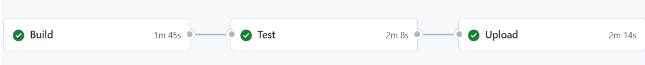
\includegraphics[width=1\textwidth]{fig/pipeline_log.png}
    \caption{Etapas del pipeline}
    \label{fig:pipeline3}
\end{figure}
\subsection{Tests}
Para implementar los tests se hace uso de \href{http://www.throwtheswitch.org/unity}{Unity Tests}, el cual es una herramienta que provee aserciones (o ``\textbf{Asserts}''), que son sentencias que verifican que se cumplan ciertas condiciones en el código. Está escrito en lenguaje C y está pensado especialmente para microcontroladores y sistemas embebidos, permite usar macros y otras facilidades para probar estos sistemas durante su desarrollo.

Dentro del proyecto, los tests se ubican en la carpeta \textbf{/test/}, en este caso se tiene sólo un archivo de tests, llamado \textbf{test\_main.c}.

Se crearon 2 tests:
\begin{enumerate}
\item Chequear que $$DELAY >= 50 [ms] $$
Para esta prueba se usa la función \textbf{TEST\_ASSERT\_GREATER\_OR\_EQUAL()}
\item Chequear que $$ DELAY <= 5000 [ms] $$
Para esta prueba se usa la función \textbf{TEST\_ASSERT\_LESS\_OR\_EQUAL()}
\end{enumerate}

A continuación se presenta el código:

\begin{lstlisting}[language=C, caption={UnityTests}, label={cod:unity-tests}, captionpos=b]
#include <unity.h>
#include "blink.h"
void test_blink_led(void)
{
  //Test if DELAY value is between 50 and 5000 ms
  TEST_ASSERT_GREATER_OR_EQUAL(50, DELAY);
  TEST_ASSERT_LESS_OR_EQUAL(5000, DELAY);
}
int runUnityTests(void)
{
  UNITY_BEGIN();
  RUN_TEST(test_blink_led);
  return UNITY_END();
}
void app_main()
{
  runUnityTests();
}
\end{lstlisting}

\textbf{Rango Válido de valores de DELAY:}
 $$50[ms] <= DELAY <= 5000[ms]$$

Estos tests crean un \textbf{rango válido de valores} para la constante de tiempo DELAY. Recordemos que \textbf{DELAY es el tiempo que tiene que transcurrir para que el LED cambie de estado}, es decir, se encienda si está apagado o viceversa. La idea es que si no se cumple alguna de estas pruebas, el pipeline no continúe su ejecución normal y se evite cargar el código en la placa, simulando una prevención de posibles daños.

\newpage
\subsection{Runners}

Cuando se trabaja con pipelines, por defecto las acciones se ejecutan en un servidor en la nube, llamado \textbf{Runner}. Si bien GitHub provee un runner de forma gratuita, está limitado a una cantidad de minutos de ejecución por mes, luego solicita un pago. A continuación se presenta la tabla \ref{tab:minutos-gratuitos} con la información de facturación de los runners de GitHub.

\begin{table}[H]
\begin{center}
\begin{tabular}{lll}
\hline
\multicolumn{1}{|l|}{\textbf{Producto}} & \multicolumn{1}{l|}{\textbf{Almacenamiento}} & \multicolumn{1}{l|}{\textbf{Minutos por mes}} \\ \hline
\multicolumn{1}{|l|}{GitHub Free} & \multicolumn{1}{l|}{500MB} & \multicolumn{1}{l|}{2000} \\ \hline
\multicolumn{1}{|l|}{GitHub Pro} & \multicolumn{1}{l|}{1GB} & \multicolumn{1}{l|}{3000} \\ \hline
\end{tabular}
\caption{Minutos Gratuitos de los GitHub Runners}
\label{tab:minutos-gratuitos}
\end{center}
\end{table}

A su vez, dependiendo del sistema operativo deseado para el runner, se tiene un multiplicador de minutos, que básicamente indica que un minuto de reloj se contabiliza como varios minutos de runner, consumiendo más rápidamente la tasa de minutos gratuitos. La tabla \ref{tab:multiplicadores-minutos} detalla los multiplicadores mencionados.

\begin{table}[H]
\begin{center}
\begin{tabular}{lll}
\hline
\multicolumn{1}{|l|}{\textbf{Sistema Operativo}} & \multicolumn{1}{l|}{\textbf{Multiplicador de Minutos}} \\ \hline
\multicolumn{1}{|l|}{Linux} & \multicolumn{1}{l|}{1} \\ \hline
\multicolumn{1}{|l|}{Windows} & \multicolumn{1}{l|}{2} \\ \hline
\multicolumn{1}{|l|}{macOS} & \multicolumn{1}{l|}{10} \\ \hline
\end{tabular}
\caption{Multiplicadores de Minutos de los GitHub Runners}
\label{tab:multiplicadores-minutos}
\end{center}
\end{table}

La facturación del runner se hace en función de cuantos minutos se sobrepasen del límite de minutos gratuitos por mes. La siguiente tabla \ref{tab:costos-minutos}

\begin{table}[H]
\begin{center}
\begin{tabular}{lll}
\hline
\multicolumn{1}{|l|}{\textbf{Sistema Operativo}} & \multicolumn{1}{l|}{\textbf{Tasa por minuto (USD)}} \\ \hline
\multicolumn{1}{|l|}{Linux} & \multicolumn{1}{l|}{\$0.008} \\ \hline
\multicolumn{1}{|l|}{Windows} & \multicolumn{1}{l|}{\$0.016} \\ \hline
\multicolumn{1}{|l|}{macOS} & \multicolumn{1}{l|}{\$0.08} \\ \hline
\end{tabular}
\caption{Costos de Minutos de los GitHub Runners}
\label{tab:costos-minutos}
\end{center}
\end{table}

(La información acerca de la facturación de GitHub Runners se encuentra en: \href{https://docs.github.com/es/billing/managing-billing-for-github-actions/about-billing-for-github-actions}{Billing for GitHub Actions})

Por este motivo es recomendable crear un Runner local, también conocido como \textbf{self-hosted runner}, es decir, brindar la capacidad de cómputo de una computadora propia para permitirle al repositorio correr las tareas o jobs, evitando usar los recursos de la nube y \textbf{tener un runner disponible de manera gratuita}.

Luego de seguir las instrucciones para levantar el runner local, se tuvo el inconveniente de que funciona en la distribución Ubuntu pero no en LinuxMint, debido a un error de dependencias de módulos de Python. Para solucionar este problema, \textbf{se corre el self-hosted runner dentro de un contenedor de Docker}, que se detalla en la siguiente sección.

\subsection{Docker}

\href{https://www.docker.com/}{Docker} es una herramienta popular en la cultura DevOps, que permite crear contenedores que encapsulan las dependencias que requiere una aplicación para correr.

Los \textbf{contenedores} son piezas de software livianas, independientes, empaquetables y ejecutables que incluyen todo lo que necesita para correr: código, runtime, herramientas de sistema, librerías y configuraciones. Cabe aclarar que un contenedor se ejecuta como un proceso independiente dentro de un sistema operativo por consiguiente puede ser afectado por el controlador de procesos del sistema operativo.

Por otro lado, una \textbf{imagen} de Docker, es una receta para poder construir contenedores, tantos contenedores como sean necesarios de la misma aplicación. Cada imagen está descrita en un archivo llamado \textbf{Dockerfile}, dentro de este archivo se encuentran todas las etapas necesarias para construir la imagen.

Hasta este punto se tiene una imagen construida y un contenedor a partir de la imagen, ejecutándose en nuestra máquina local. Sin embargo, la potencia de los contenedores se presenta a la hora de realizar despliegues (o ``Deployments'') con ellos. Para esto añadimos un nuevo concepto llamado \textbf{registro}. \textbf{Docker registry} es un repositorio de artefactos donde podemos almacenar imágenes de Docker. La versión comercial se encuentra en \href{https://hub.docker.com}{Dockerhub}.

La figura \ref{fig:docker} muestra un esquema en el que se ilustran los conceptos mencionados, además de los comandos de Docker, y aparece el Docker daemon, que es el proceso encargado de gestionar las imágenes y contenedores. Por otro lado, el registry representa un repositorio en la nube, al que se pueden subir o bajar imágenes.

\begin{figure}[H]
    \centering
    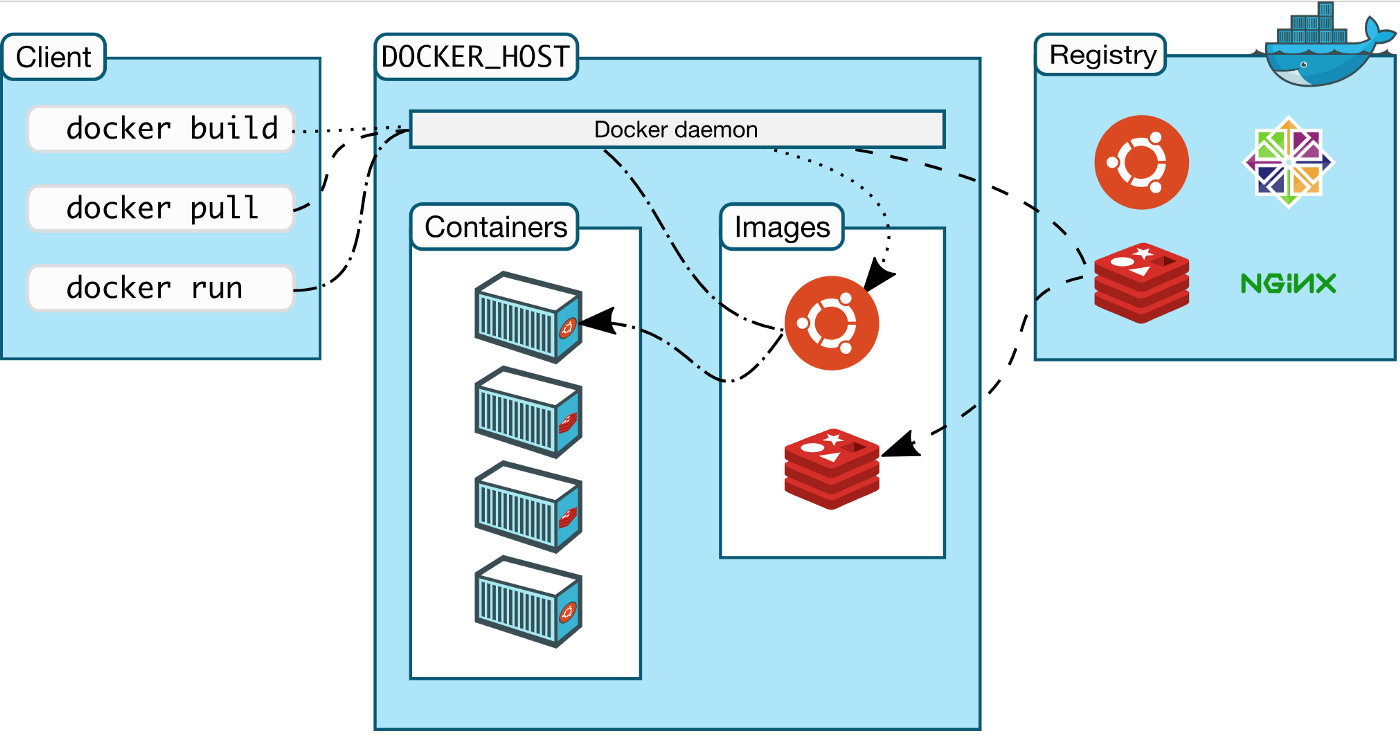
\includegraphics[width=1\textwidth]{fig/docker.png}
    \caption{Docker: Esquema de los conceptos}
    \label{fig:docker}
\end{figure}

(La figura \ref{fig:docker} es propiedad intelectual de Mauricio Collazos, y su post se encuentra en este \href{https://medium.com/ingenier%C3%ADa-en-tranqui-finanzas/una-gu%C3%ADa-no-tan-r%C3%A1pida-de-docker-y-kubernetes-933f5b6709df } {enlace} )

Gracias a la tecnología de los contenedores, podemos abstraernos del sistema en el  que se corre la aplicación, y dar solución al problema de que la aplicación funciona en algunos sistemas y no en otros, típicamente por problemas en sus dependencias.

En concreto, se partió de la imagen \href{https://registry.hub.docker.com/r/tcardonne/github-runner}{GitHub Runner de TCardonne} para crear un \textbf{self-hosted runner pero esta vez encapsulado en un contenedor}.

\subsubsection{Docker Compose}

Para facilitar la inicialización del contenedor se usa \href{https://docs.docker.com/compose/}{Docker Compose}, que es una herramienta para declarar como código YAML uno o más contenedores para instanciarse, desde qué imagen se parte, y su configuracion específica, como el mapeo de puertos con el sistema host, si posee o no un volumen asociado, entre otras. 

Gracias a esta herramienta, basta con ejecutar el comando \textbf{sudo docker-compose up} para iniciar el contenedor correspondiente al self-hosted runner. Cabe aclarar que Docker Compose no agrega funcionalidad más allá de Docker, sino que permite declarar como código las configuraciones que de otra forma tendrían que hacerse con los comandos de docker: \textbf{docker pull, docker build, docker run} como se muestran en la figura \ref{fig:docker}. Este código se encuentra en el archivo \href{https://github.com/FeedehC/pipeline-esp32/blob/main/docker-compose.yml}{docker-compose.yml} ubicado en el directorio raíz del proyecto.

Una vez que está corriendo el contenedor de Docker con el self-hosted runner, el mismo está ``escuchando jobs", lo que significa que está a la espera de que un evento dispare la ejecución del pipeline, es decir, que un desarrollador haga un push que involucre cambios en el código, en este caso un cambio en la frecuencia de intermitencia del LED.

A continuación se presenta una captura de pantalla de la terminal que corre el contenedor con el runner, en la figura \ref{fig:runner}.

\begin{figure}[H]
    \centering
    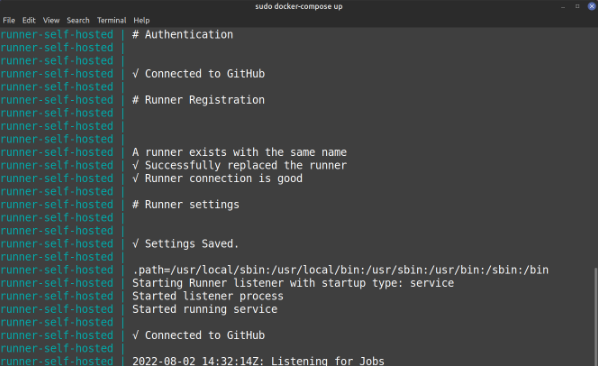
\includegraphics[width=1\textwidth]{fig/runner_log.png}
    \caption{GitHub Self-Hosted Runner}
    \label{fig:runner}
\end{figure}


\subsection{Documentación}
Una vez logrado el pipeline y su ejecución exitosa, se documentó el trabajo, confeccionando el presente informe de las actividades llevadas a cabo, y además el README del \href{https://github.com/FeedehC/pipeline-esp32}{repositorio de GitHub} que indica paso a paso como crear un repositorio personal con el proyecto, es decir, un \textbf{``fork''}, y como implementar el pipeline para un proyecto personal. 

Si bien el proyecto está configurado para trabajar con una placa \textbf{ESP32 tipo NodeMCU32s}, en caso que otros desarrolladores necesiten implementar el pipeline para un proyecto que usa otro dispositivo, en caso que el dispositivo sea soportado por PlatformIO (lo que se puede verificar en el siguiente \href{https://registry.platformio.org/search?t=platform}{enlace}), bastará con ajustar las configuraciones en el archivo \href{https://github.com/FeedehC/pipeline-esp32/blob/main/platformio.ini}{\textbf{platformio.ini}} ubicado en la carpeta raíz del repositorio. Es en este archivo donde se detallan los ajustes para PlatformIO y es posible incluso declarar más de un entorno de trabajo, es decir, trabajar con distintos dispositivos e indicar qué dependencias corresponden a cada uno. 

Para subir el código a un dispositivo u otro, se debe aclarar el \textbf{environment} al momento de ejecutar el comando \textbf{pio run}, típicamente en el archivo \href{https://github.com/FeedehC/pipeline-esp32/blob/main/.github/workflows/main.yml}{\textbf{.github/workflows/main.yml}}, es decir, en el código yaml del pipeline.

Como extra \textbf{se añadió una versión en inglés de la documentación} del repositorio, que se puede encontrar en el archivo \href{https://github.com/FeedehC/pipeline-esp32/blob/main/README-english.md}{\textbf{README-english.md}} en la raíz del repositorio, con el propósito de poder compartirlo con desarrolladores que prefieran esta lengua para trabajar.

